
Систематические ошибки, вызванные физическими неидеальностями
ускорителя, включая неточность юстировки оптических элементов,
вызывают фальш-сигнал ЭДМ.~\cite[стр.~230]{Eremey:Thesis} Особенно в
этом отношении проблематичны наклоны элементов вокруг оптической оси, поскльку они
индуцируют паразитные горизонтальные компоненты магнитного поля $B_x$
и $B_z$, которые обе вращают спин в вертикальной плоскости; той, в которой измеряется ЭДМ.

Ю. Сеничевым были сделаны~\cite{Senichev:FDM} аналитические оценки МДМ частоты прецессии спина
вокруг радиальной оси. Из уравнения Т-БМТ, и выражения силы Лоренца,
скорость МДМ прецессии вокруг радиальной оси есть
\begin{equation}
\SD{\W_x^{MDM}} = \frac{q}{m\gamma}\frac{G+1}{\gamma}\frac{\SD{B_x}}{\sqrt{n}},
\end{equation}
где $n$ есть число наклонённых спин-ротаторов, и $\SD{B_x} = B_y
\SD{\delta h}/L$, при стандартном отклонении ошибки юстировки
$\SD{\delta h}$. При величине ошибки $\SD{\delta h} = 100$ мкм, и
длине дефлектора $L=1$ м, $\SD{\W_x^{MDM}} \approx 100$ рад/сек.~\cite{Senichev:FDM}

Мы изучили спиновую динамику в структурах с замороженным и
квази-замороженным спином в присутствии наклонов оптических элементов
с помощью кода COSY INFINITY. Наши симуляции согласуются с оценками,
представленными выше.

\paragraph{Имплементация паразитного поля.}\label{sec:error_field_implementation}
Имплементируя неидеальности полей, мы следовали рекомендациям
изложенным в~\cite[стр.~235]{Eremey:Thesis}. Малое возмущение
магнитного поля, в первом приближении, действует как маленький пропорциональный поворот
спин-вектора. Поэтому мы имплементировали наклон E+B элемента как
домножение соответствующей матрицы поворота на его спиновую матрицу
перехода, ``спин-кик.''

В соответствии с уравнением~\eqref{eq:TBMT_MDM}, изменение МДМ частоты
прецессии, ассоциированное с введённым паразитным полем $(B_x, 0, B_z)$ есть
\begin{align*}
	\Delta\W_{MDM} &= \frac qm (B_x, 0, B_z),
	\intertext{поэтому угол спин-кика равен}
	\Theta_{kick} &= t_0\Delta\W_{MDM},
\end{align*}
где $t_0 = L/v_0$ пролётное время референсной частицы через элемент.

\subsection{Зависимость от распределения неидеальностей} \label{sec:simulation-fake_signal}
Данная серия симуляций была проведена с целью подтвердить два тезиса
касательно систематической ошибки измерения частоты прецессии спина в
вертикальной плоскости, вызванной неточностью установки E+B элементов:
\begin{enumerate*}[1)]
	\item индуцированный МДМ-эффект зависит только от среднего значения
	угла наклона элементов, но не от  конкретной последовательности
	углов (т.е. отсутствует эффект \emph{геометрической фазы}); и
	\item эта зависимость носит линейный характер.
\end{enumerate*}

Наклон элемента вокруг оптической оси моделировался путём добавления
после элемента спин-кика вокруг радиальной оси соответствующей
величины (см. раздел~\ref{sec:error_field_implementation}). Это
гарантирует сохранение замкнутой орбиты при введении наклонов, что
физически обусловлено появлением компенсирующего электрического поля 
спин-ротатора при его наклоне.

Симуляция была проведена следующим образом: мы распределили наклоны
$\Theta_{tilt}$ E+B элементам FS структуры случайным образом. После
построения матриц перехода 3-го порядка, были вычислены разложения
Тейлора функций спин-тюна и оси прецессии спина (SPA). Члены нулевого
порядка этих разложений представляют собой спин-тюн и SPA референсной частицы.

Симуляция была проведена 11 раз; каждый раз углы наклона
спин-ротаторов выбирались из нормального распределения
$N(\mu_0\cdot(i-5), \sigma_0)$, где $\mu_0 = 10\cdot \sigma_0 =
10^{-4}$ рад, $i\in\lbrace0,\dots, 10\rbrace$. Результаты представлены
на Рисунке~\ref{fig:Linearity_test_shifting_gauss}.

\begin{figure}[!h]
	\centering\hfill
	\subbottom[Компоненты оси прецессии.]{%
		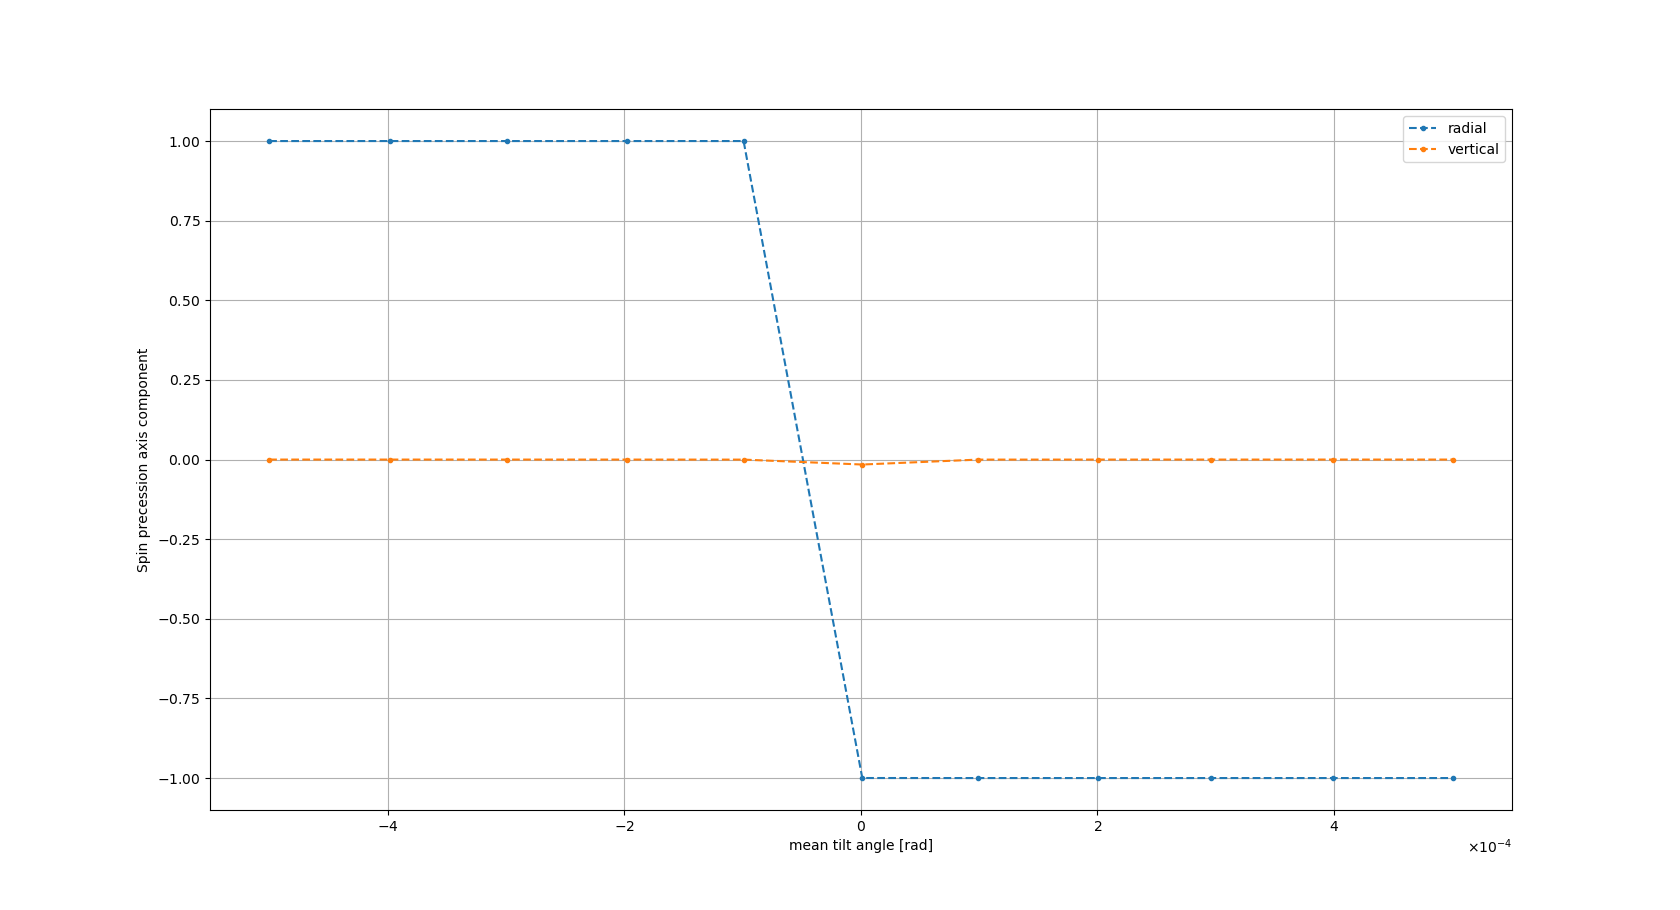
\includegraphics[width=\textwidth]{images/fake_signal_sim/linearity_test_shifting_gauss_nbar}}
	\hfill
	\subbottom[Компоненты частоты прецессии.]{%
		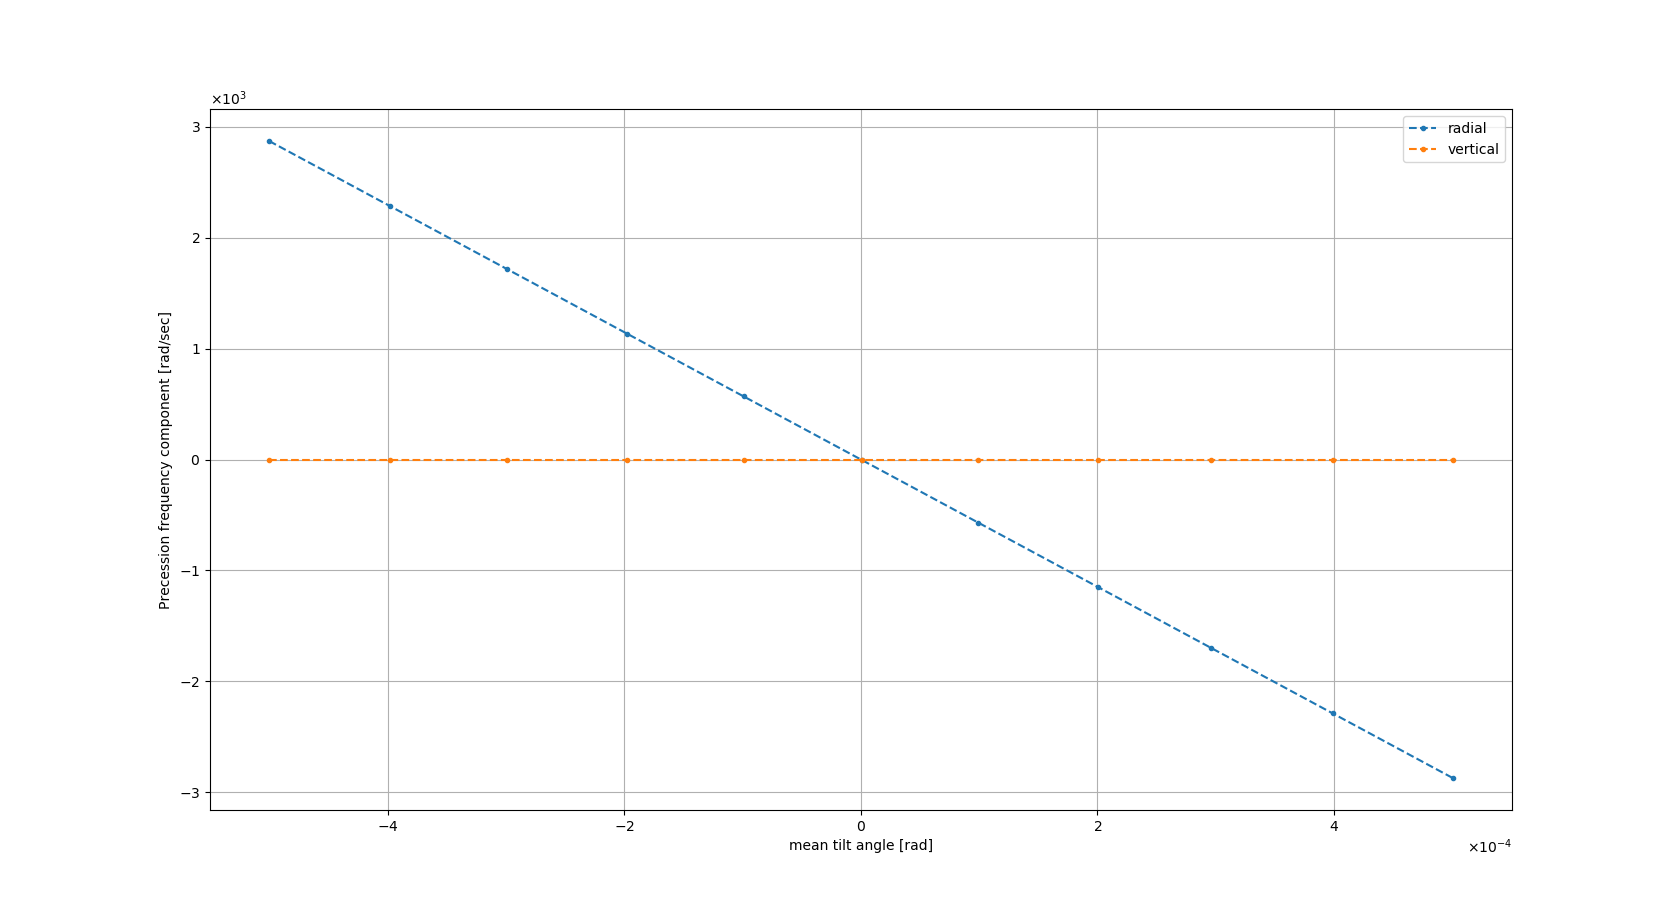
\includegraphics[width=\textwidth]{images/fake_signal_sim/linearity_test_shifting_gauss_freq}}
	\hfill
	\legend{Цветом различаются радиальная (синий) и вертикальная (оранжевый) компоненты векторов $\bar n$, $\vec\W$.}
	\caption{Зависимость направления и частоты прецессии спина референсной частицы в неидеальной FS-структуре со случайно распределёнными ошибками установки спин-ротаторов от их среднего угла наклона. (Случайно распределённая ошибка установки.)\label{fig:Linearity_test_shifting_gauss}}
\end{figure}

На Рисунке~\ref{fig:Linearity_test_compensated} изображены результаты теста, в котором E+B элементы попарно повёрнуты на противоположные углы (три случайные пары), а один элемент повёрнут на угол
$\mu_i = (i-5)\cdot 10^{-6}$ рад, $i\in\lbrace0,\dots,10\rbrace$. Обе симуляции были выполнены на энергии
270.0092 МэВ.\footnote{На этой энергии ось прецесии спина и спин-тюн
	не определены в системе координат связанной с пучком, использованной
	COSY INFINITY, для идеальной структуры. Это соответствует ситуации
	когда спин не прецессирует ни в какой плоскости (горизонтальной или
	вертикальной), что есть условие замороженного спина в идеальной структуре.}

\begin{figure}[!h]
	\centering\hfill
	\subbottom[Компоненты оси прецессии]{%
		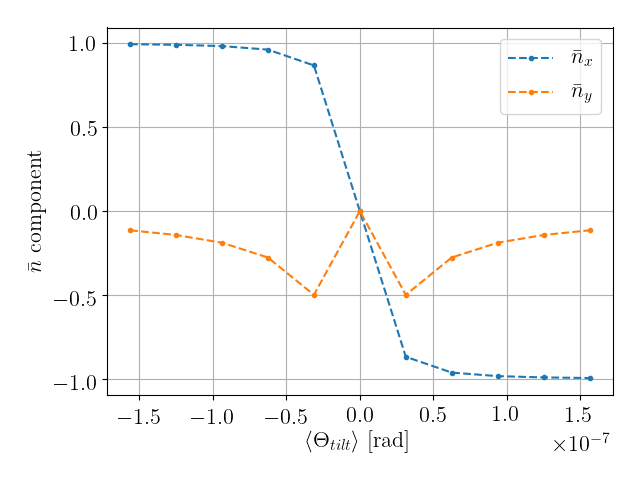
\includegraphics[width=\textwidth]{images/fake_signal_sim/linearity_test_compensated+microrad_nbar}}
	\hfill
	\subbottom[Компоненты частоты прецессии]{%
		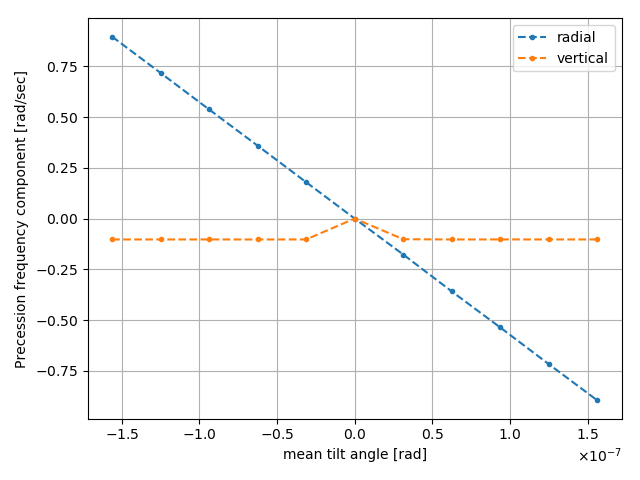
\includegraphics[width=\textwidth]{images/fake_signal_sim/linearity_test_compensated+microrad_freq}}
	\hfill
	\legend{Цветом различаются радиальная (синий) и вертикальная (оранжевый) компоненты векторов $\bar n$, $\vec\W$.}
	\caption{Зависимость направления и частоты прецессии спина референсной частицы в неидеальной FS-структуре со случайно распределёнными ошибками установки спин-ротаторов от их среднего угла наклона. (Скомпенсированная ошибка установки.)\label{fig:Linearity_test_compensated}}
\end{figure}

\subsection{Равенство частот прецессии спинов частиц при движении в прямом и обратном направлениях}
TODO